\documentclass[slidestop,mathserif]{beamer}

\usetheme{Madrid}
\usecolortheme{seahorse}

\usepackage{geometry}
\usepackage{graphicx}
\usepackage{amssymb}
\usepackage{epstopdf}
\usepackage{amsmath}  	% this permits text in eqnarray among other benefits
\usepackage{color}          	% gives color options
\usepackage{url}		% produces hyperlinks
\usepackage[english]{babel}
\usepackage[latin1]{inputenc}
\usepackage{colortbl}	% allows for color usage in tables
\usepackage{multirow}	% allows for rows that span multiple rows in tables
\usepackage{xcolor}		% this package has a variety of color options
\usepackage{calc}
\usepackage{multicol}

\setbeamertemplate{navigation symbols}{}

%User defined colors: See colors section
\xdefinecolor{oiBlue}{rgb}{0.15, 0.35, 0.55}
\xdefinecolor{gray}{rgb}{0.5, 0.5, 0.5}
\xdefinecolor{darkGray}{rgb}{0.3, 0.3, 0.3}
\xdefinecolor{darkerGray}{rgb}{0.2, 0.2, 0.2}
\xdefinecolor{rubineRed}{rgb}{0.89,0,0.30}
\xdefinecolor{linkCol}{rgb}{0.11,0.49,0.95}	
\xdefinecolor{irishGreen}{rgb}{0,0.60,0}	
\xdefinecolor{darkturquoise}{rgb}{0.44, 0.58, 0.86}
\definecolor{lightGreen}{rgb}{0.533,0.765,0.42}

\setbeamercolor*{palette primary}{fg=white,bg= oiBlue!70}
\setbeamercolor*{palette secondary}{fg=black,bg= oiBlue!20!white}
\setbeamercolor*{palette tertiary}{fg=white,bg= oiBlue!80!black!90}
\setbeamercolor*{palette quaternary}{fg=white,bg= oiBlue}

\setbeamercolor{structure}{fg= oiBlue}
\setbeamercolor{frametitle}{bg= oiBlue!70}

\setbeamercolor{disc body}{bg=oiBlue!20!white!80,fg=oiBlue!80!black!90}
\setbeamercolor{disc title}{bg=oiBlue!40!white!60,fg=oiBlue!70!black!100}


\setbeamertemplate{blocks}[shadow=false]


\newcommand{\removepagenumbers}{% 
  \setbeamertemplate{footline}{
    %
    \begin{beamercolorbox}[colsep=1.5pt]{upper separation line foot}
    \end{beamercolorbox}
    \begin{beamercolorbox}[ht=2.5ex,dp=1.125ex,%
      leftskip=.3cm,rightskip=.3cm plus1fil]{author in head/foot}%
      \leavevmode{\usebeamerfont{author in head/foot}\insertshortauthor}%
%      \hfill%
%      {\usebeamerfont{author in head/foot}\usebeamercolor[fg]{institute in head/foot}\insertshortinstitute}%
    \end{beamercolorbox}%
    \begin{beamercolorbox}[ht=2.5ex,dp=1.125ex,%
      leftskip=.3cm,rightskip=.3cm plus1fil]{title in head/foot}%
      {\usebeamerfont{title in head/foot}\insertshorttitle}%
      \hfill%
      {\usebeamerfont{author in head/foot}\usebeamercolor[fg]{institute in head/foot}\insertshortinstitute}%
    \end{beamercolorbox}%
    \begin{beamercolorbox}[colsep=1.5pt]{lower separation line foot}
    \end{beamercolorbox}
    }
} 


\newcommand{\disc}[2]{
\begin{beamerboxesrounded}[shadow = true, lower = disc body, upper = disc title]{#1}
#2
\end{beamerboxesrounded}
}


\AtBeginSection[] 
{ 
  \addtocounter{framenumber}{-1} 
  % 
  {\removepagenumbers 
    \begin{frame}<beamer> 
    \tableofcontents[currentsection] 
  \end{frame} 
  } 
} 

\usepackage{isotope}
\usepackage{bm}
\usepackage{minted}

\title[JSM 2012]{Leveraging GPU Libraries for Efficient Computation of Bayesian Spatial Assignment Models in R}
\author{Colin Rundel}
\date{August 1, 2012}
\institute[UCLA / Duke]{University of California, Los Angeles / Duke University}


\begin{document}

\begin{frame}[plain]
\titlepage
\end{frame}

%==================================================================================================
%==================================================================================================

\section{Background}
\addtocounter{framenumber}{-1} 

%==================================================================================================

\begin{frame}
\frametitle{Project Background}

Developing methods to make use of intrinsic markers (genetic and isotopic signals) for the purpose of inferring migratory connectivity.

\begin{itemize}
\item Existing methods are too coarse for most applications
\item Large amounts of data are available ( \textgreater{}150,000 feather samples from \textgreater{}500 species)
\item Genetic assignment methods are based on Wasser, et al. (2004)
\item Isotopic assignment methods are based on Wunder, et al. (2005)
\end{itemize}

\vspace{3mm}

Preliminary Data (microsats and $\delta \isotope[2]{H}$):
\begin{itemize}
\item Hermit Thrush (\textit{Catharus guttatus}) - 138 Individuals, 14 Locations, 6 Loci, 9-27 Alleles
\item Wilson's Warbler (\textit{Wilsonia pusilla}) - 163 Individuals, 8 Locations, 9 Loci, 15-31 Alleles
\end{itemize}


\end{frame}


%==================================================================================================
%==================================================================================================

\section{Model}

\begin{frame}
\frametitle{Allele Frequency Model}

For the allele $i$, from locus $l$, at location $k$

\begin{align*}
\bm{y_{l \cdot k}} \sim \text{MN}\left(n_{lk}=\textstyle\sum_i y_{lik}, \bm{f_{l \cdot k}}\right) \\
\\
f_{lik} = \frac{\exp(X_{lik})}{\sum_i \exp(X_{lik})} \quad
\bm{X}_{li} \sim \mathcal{N}( \bm{M}_{li}, \bm{\Sigma_{}})
\end{align*}

\pause

Likelihood:
\begin{align*}
       &~\prod_l \prod_k \frac{n_{lk}!}{\prod_i y_{lik}!} \textstyle\prod_i (f_{lik})^{y_{lik}} \\
\times &~\prod_l \prod_i 2\pi^{-r/2} |\bm\Sigma|^{-1/2} \exp\left[ -\frac{1}{2}(\bm{X_{li}} - \bm{M}_{li})'\bm\Sigma^{-1} (\bm{X_{li}} - \bm{M}_{li}) \right]\\
\times &~\pi(\bm\theta)
\end{align*}

\end{frame}

%==================================================================================================

\begin{frame}
\frametitle{Implementation}

Model fitting and prediction is done via MCMC
\begin{itemize} \addtolength{\itemsep}{3mm}
\item Original implementation in pure C++ with minimal dependencies
\item Rewritten using R / C++ via Rcpp(Armadillo) 
\begin{itemize}
\item Code closer to matrix notation (and R)
\item Transparent use of high performance LAPACK implementations (ATLAS, OpenBLAS, Intel MKL)
\end{itemize}
\item GPU based optimizations were added using CUDA, CUBLAS, and MAGMA libraries
\item Cross platform R package scatR (hopefully added to CRAN soon)
\end{itemize}

\end{frame}


%==================================================================================================
%==================================================================================================

\begin{frame}
\frametitle{Performance}

{\small System specs - 4 core Intel i5-2500K, GeForce GTX 460} \\
{\small Software specs - Ubuntu 12.04, ATLAS 3.8.4, Cuda 4.2, Magma 1.1} \\
~\\
\pause

Performance during model fitting is quite good... \\

\begin{center}
100,000 iterations in $\sim 45$ seconds
\end{center}

\pause 

Performance during prediction is much slower... \\
\begin{center}
100,000 iterations in $\sim 2580$ seconds (43 mins) \\
(predictions calculated every 100 iterations)
\end{center}

\pause

Not too bad in the greater scheme of things, but we would really like to be able to do cross validation ($\sim 200$ runs per species) ...

\end{frame}

%==================================================================================================

\begin{frame}
\frametitle{Prediction Example}

\begin{center}
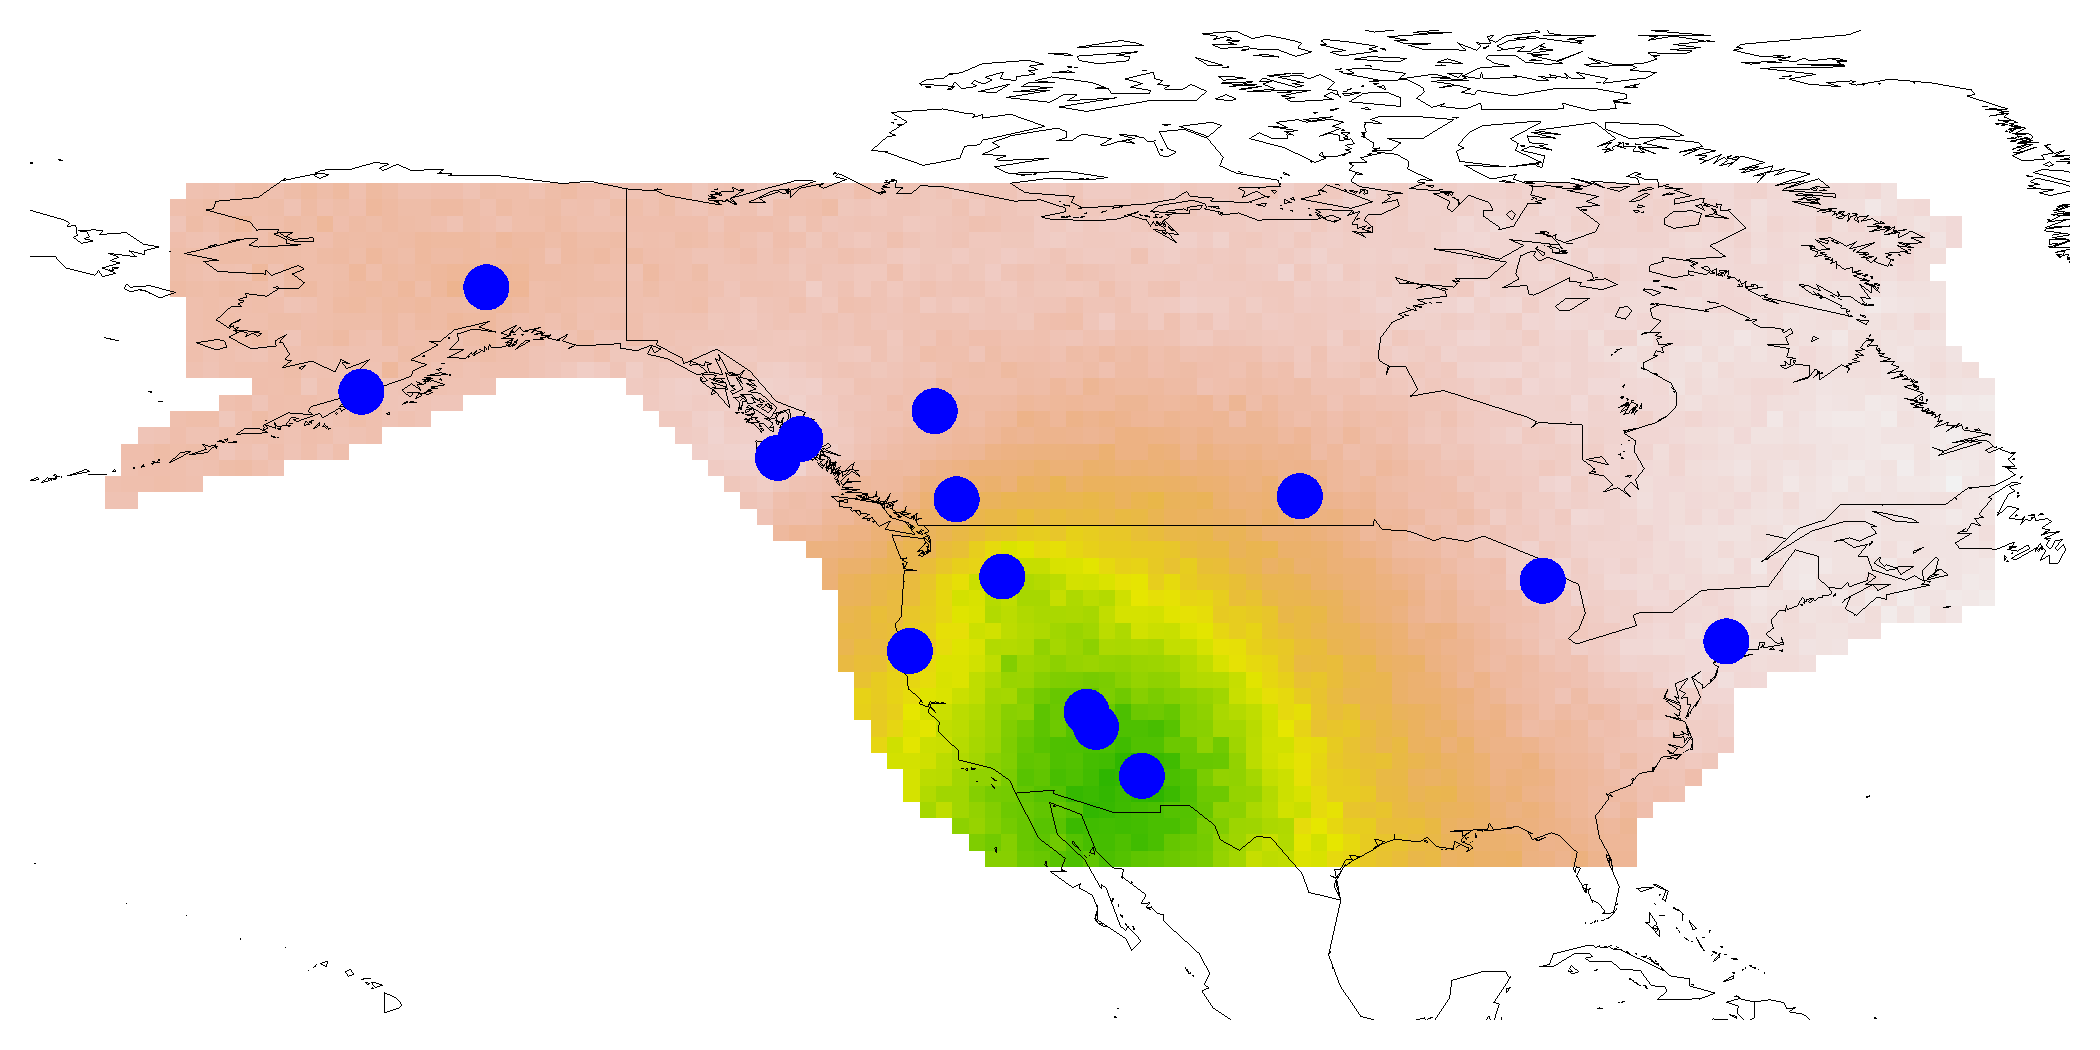
\includegraphics[width=0.9\textwidth]{pics/HETH_Al3-1.pdf}
\end{center}
\end{frame}

%==================================================================================================

\begin{frame}
\frametitle{Prediction algorithm details}

Why is the prediction slow? \pause We are predicting allele frequencies for Hermit thrush at 3318 novel locations.\\
~\\
To do so we need to draw samples from:
\[ \bm{X_p} | \bm{X_m} \sim \mathcal{N}(\bm{\mu_p}+\bm\Sigma_{pm}\bm\Sigma_{m}^{-1}(\bm{X_m}-\bm\mu_m),~ \bm\Sigma_{p}-\bm\Sigma_{pm}\bm\Sigma_{m}^{-1}\bm\Sigma_{mp}) \]

\pause

\vspace{-7mm}

\begin{columns}
\column{0.20\textwidth}
\column{0.60\textwidth}
\begin{block}{Algorithm steps}
\begin{enumerate}
\item Calculate $\bm\Sigma_{pm}$ and $\bm\Sigma_{p}$
\item Calculate $\bm\Sigma_{pm} \bm\Sigma_{m}^{-1}$
\item Calculate $\text{Chol}(\bm\Sigma_{p}-\bm\Sigma_{pm}\bm\Sigma_{m}^{-1}\bm\Sigma_{mp})$
\item Sample from MVN
\item Calculate allele frequencies
\item Output results
\end{enumerate}
\end{block}
\column{0.2\textwidth}
\end{columns}
\end{frame}

%==================================================================================================

\begin{frame}
\frametitle{Prediction algorithm timings}

\vfill

\begin{center}
\only<1>{
\begin{tabular}{|rl|c|}
\hline
& Step                                    & CPU Timing (secs)  \\
\hline                                                   
1. & Covariances                          & 1.02               \\
2. & $\bm\Sigma_{21} \bm\Sigma_{11}^{-1}$ & 0                  \\
3. & Cholesky                             & 1.15               \\
4. & Sample from MVN                      & 0.23               \\
5. & Allele Freq                          & 0.14               \\
6. & Output                               & 0                  \\
\hline
   & Total                                & 2.54               \\
\hline
\end{tabular}
}

\only<2>{
\begin{tabular}{|rl|c|c|}
\hline
& Step                                    & CPU Timing (secs)  & CPU+GPU (secs) \\
\hline
1. & Covariances                          & 1.02               & 0.05 \\
2. & $\bm\Sigma_{21} \bm\Sigma_{11}^{-1}$ & 0                  & 0    \\
3. & Cholesky                             & 1.15               & 0.23 \\
4. & GP Sample                            & 0.23               & 0.06 \\
5. & Allele Freq                          & 0.14               & 0.14 \\
6. & Write                                & 0                  & 0    \\
\hline
   & Total                                & 2.54               & 0.48 \\
\hline
\end{tabular}
}
\end{center}

\vfill

\end{frame}

%==================================================================================================

\begin{frame}
\frametitle{Improving the Cholesky step}

Not surprising given Cholesky factorization is $\mathcal{O}(n^3)$ and $n=3318$.\\
~\\
There isn't a magical solution to this, so we just want to use the fastest possible implementation of the Cholesky decomposition.

\begin{itemize}
\item \textbf{Intel MKL / OpenBLAS / Eigen} - all (multicore) CPU based with very marginal improvement 
\item \textbf{CUBLAS} - part of NVidia's CUDA toolkit, implements core BLAS functions (but not cholesky) 
\item \textbf{CULA} - proprietary / closed source (dense and sparse) GPU linear algebra library with an expensive license
\item \textbf{MAGMA} - open source Multicore+GPU dense linear algebra library (CUDA and OpenCL implementations)
\end{itemize}

\end{frame}

%==================================================================================================

\begin{frame}
\frametitle{Cholesky GPU}

\vfill
\begin{center}
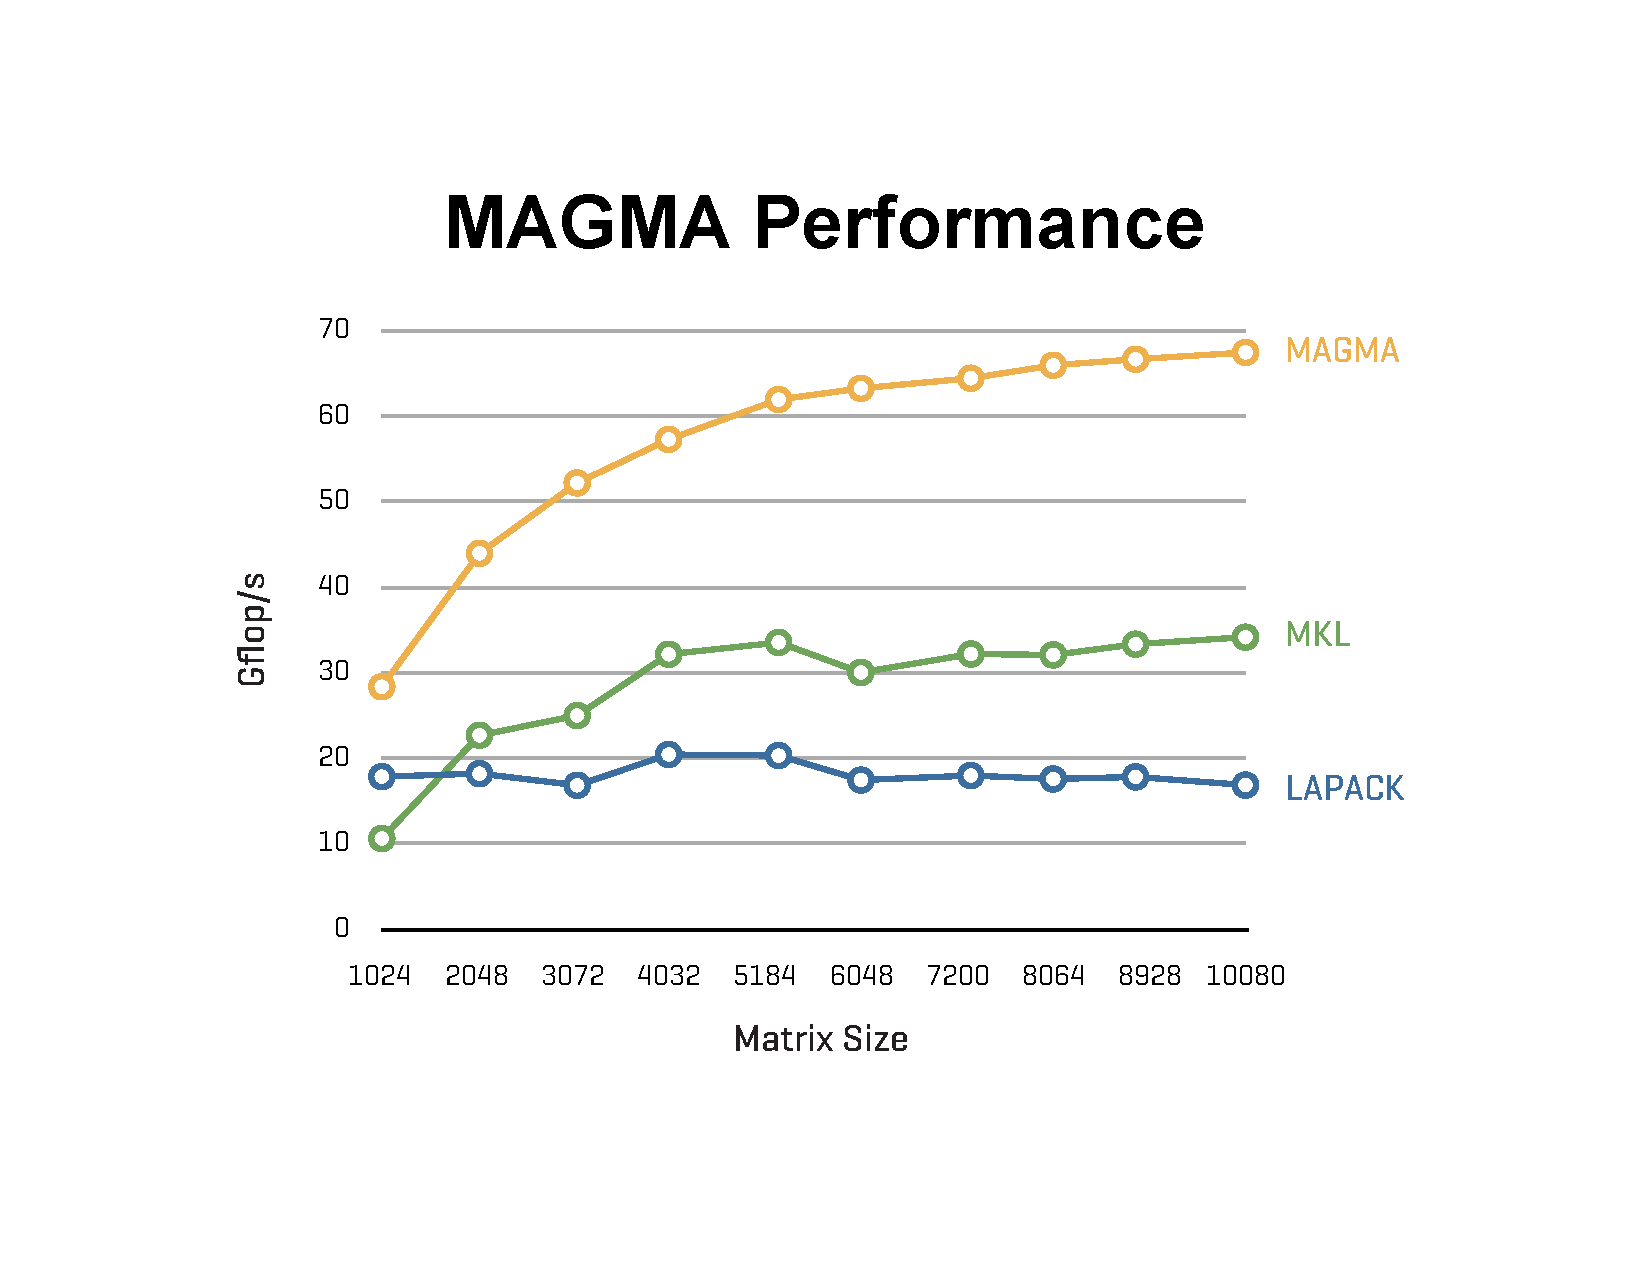
\includegraphics[width=0.7\textwidth]{pics/magma_chol.pdf}
\end{center}
\vfill
{\tiny Ltaief, H. ``A Scalable High Performant Cholesky Factorization for Multicore with GPU Accelerators''\\ VECTAR'10 Presentation, Berkeley, CA, June 22-25, 2010.}
\end{frame}

%==================================================================================================

\begin{frame}[fragile]
\frametitle{Additional Considerations}

\begin{itemize}
\item There are costs for moving data on to and off of the GPU
\item Once the data is there, may as well do as many calculations as possible
\begin{itemize}
\item Drawing sample from the GP is sped up by performing the matrix multiplication on the GPU
\end{itemize}
\item GPU code is much more verbose / dense
\end{itemize}

\pause

{\scriptsize
\begin{columns}
\column{0.0125\textwidth}
\column{0.45\textwidth}
\begin{block}{Armadillo}
\begin{minted}{c++}
arma::mat tmp = cov12.t() * p.Sinv
\end{minted}
\end{block}
\column{0.025\textwidth}
\column{0.475\textwidth}
\begin{block}{GPU (CUBLAS)}
\begin{minted}{c}
cublasDgemm_v2( 
    p.handle, CUBLAS_OP_T, CUBLAS_OP_N,
    n_pred, n_known, n_known,
   &one,
    p.d_cov12, n_known,
    p.d_invcov11, n_known,
   &zero,
    p.d_tmp, n_pred
)
\end{minted}
\end{block}
\column{0.0125\textwidth}
\end{columns}
}

\end{frame}

%==================================================================================================

\begin{frame}[fragile]
\frametitle{Improving Covariance calculations}

Covariance in our model is assumed to be stationary and isotropic (depend only on distance between locations)
\begin{itemize}
\item Elements of the covariance matrix can be calculated independently
\item Small scale ``embarrassingly parallel'' $\Rightarrow$ good candidate for the GPU.
\item Implementation is straight forward
\end{itemize}


\pause

\begin{block}{}
{\scriptsize
\begin{minted}{c}
__global__ void powered_exponential_kernel(double* dist, double* cov,
                                           const int n, const int nm,
                                           const double sigma2, const double phi,
                                           const double kappa, const double nugget) 
{
    int n_threads = gridDim.x * blockDim.x;
    int pos = blockDim.x * blockIdx.x + threadIdx.x;

    for (int i = pos; i < nm; i += n_threads)
        cov[i] = sigma2 * exp(-pow(dist[i] / phi, kappa)) + nugget*(i%n == i/n);
}
\end{minted}
}
\end{block}

\end{frame}

%==================================================================================================

\begin{frame}
\frametitle{Summary}

Relatively small changes in one function resulted in $\sim 5$x improvement
\begin{itemize}
\item Cross validation results in days and not weeks
\item Started with trying to find an improved Cholesky decomposition, other optimizations followed
\item GPU implementation was relatively painless
\item Libraries are under active development (read: things can and will break)
\item External libraries make package development non-trivial
\end{itemize}

\end{frame}

%==================================================================================================

\begin{frame}
\frametitle{Questions, Comments?}
\vfill
\begin{center}
{\Large
\renewcommand*\arraystretch{1.5}
\begin{tabular}{lll}
email        & : & rundel@gmail.com \\
github       & : & {\normalsize \urlwofont{http://github.com/rundel/}} \\
presentation & : & {\normalsize \urlwofont{http://github.com/rundel/Presentations/}} \\
\end{tabular}
}
\end{center}
\vfill
\end{frame}


%\section{Supplementary}
%
%\begin{frame}
%\only<1>{
%\frametitle{Sampling Locations (Hermit Thrush)}
%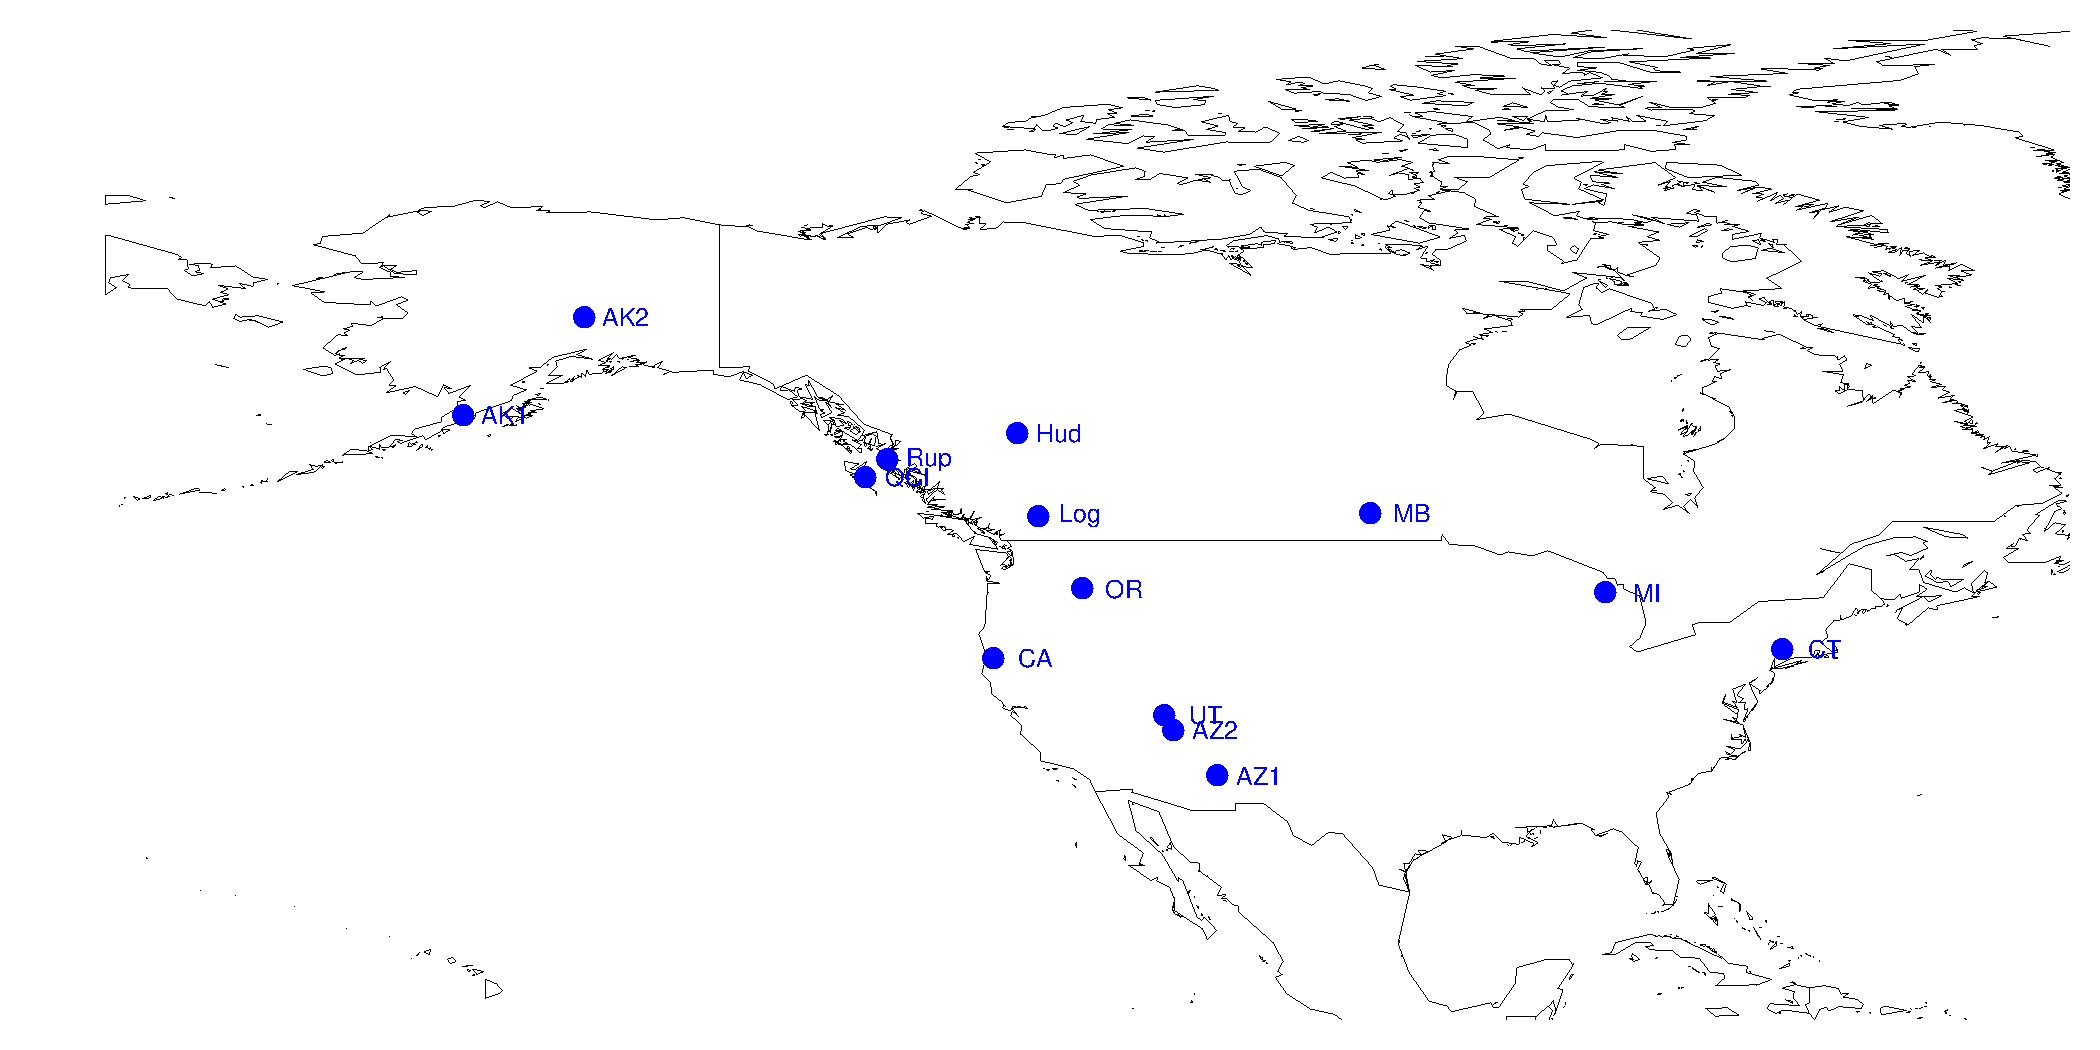
\includegraphics[width=\textwidth]{pics/HETH_locs.pdf}
%}
%\only<2>{
%\frametitle{Sampling Locations (Wilson's Warbler)}
%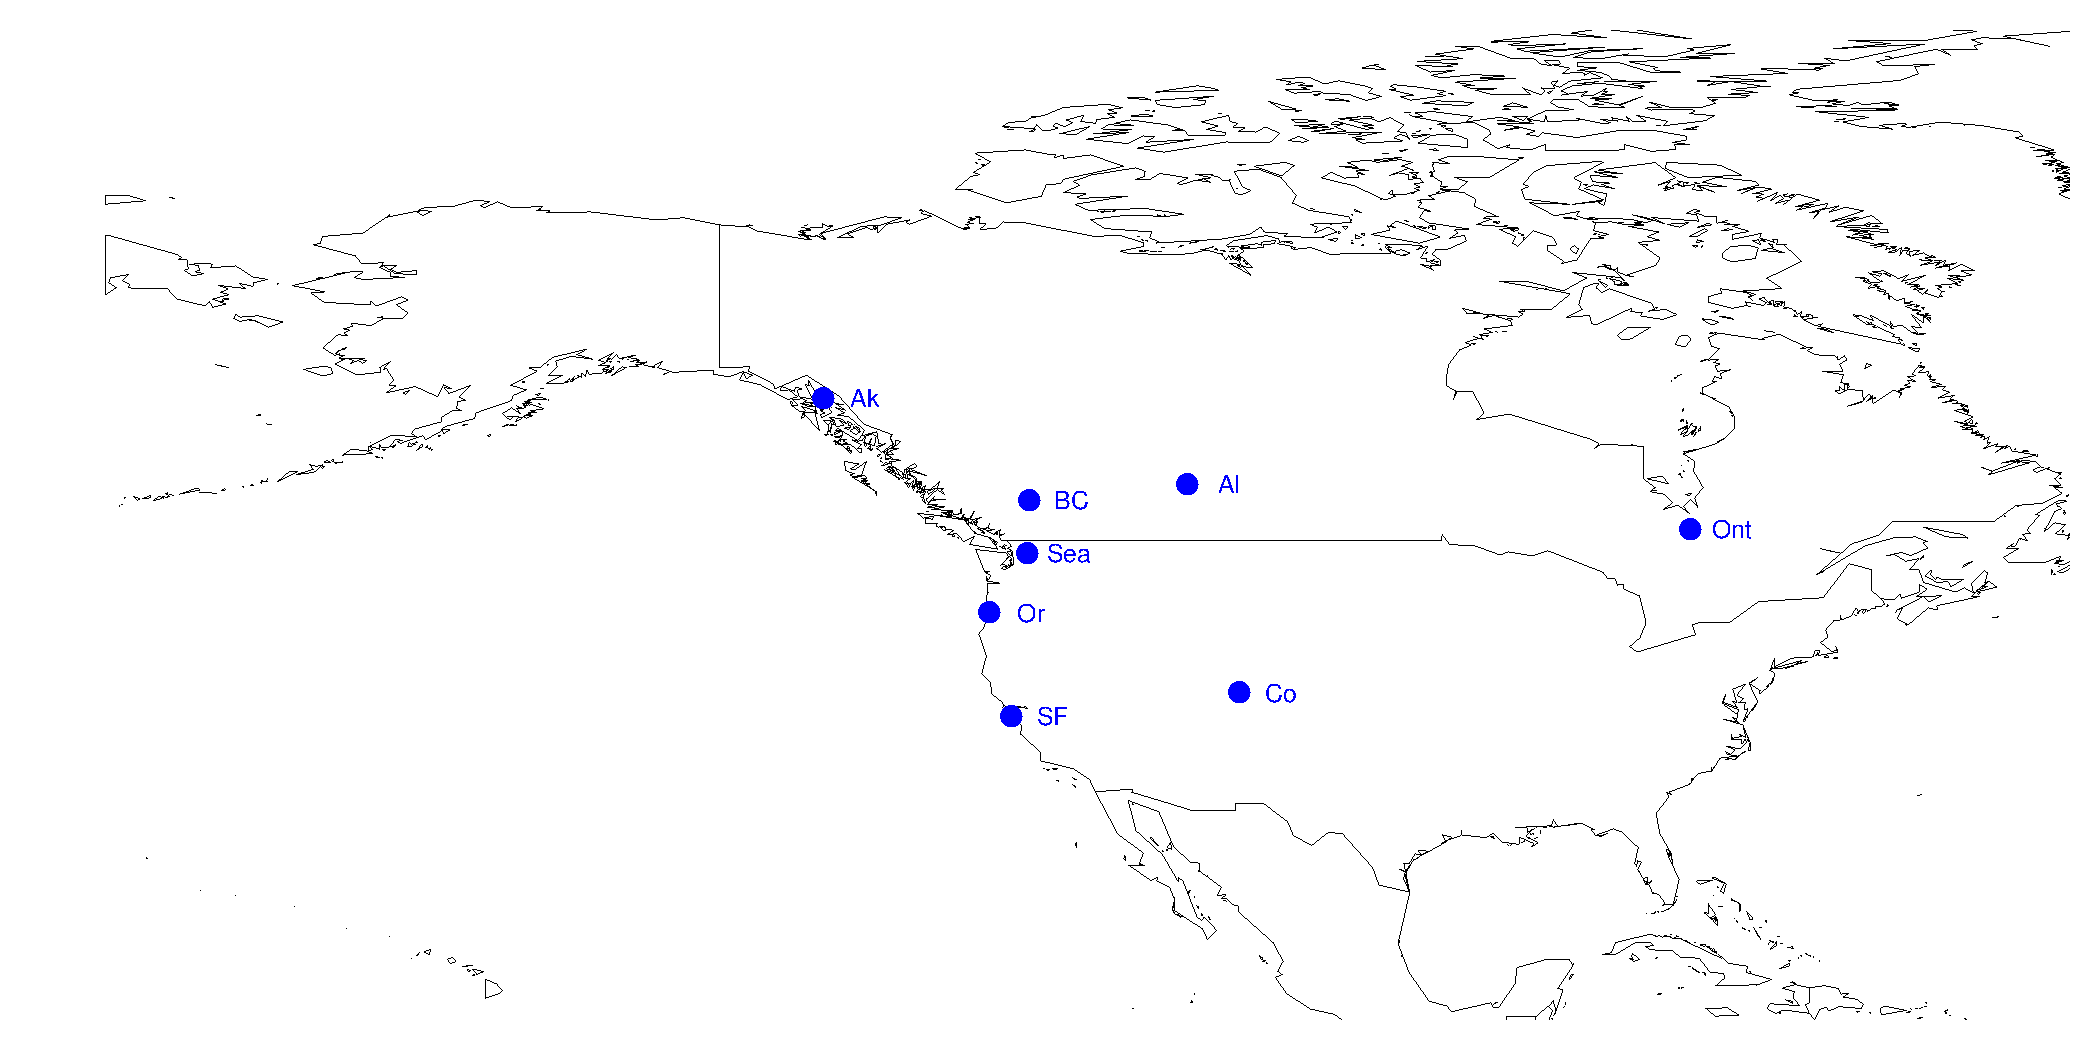
\includegraphics[width=\textwidth]{pics/WIWA_locs.pdf}\\
%}
%\end{frame}

\end{document}